\colorsection{Potencial eléctrico}
\setcounter{figure}{0}
%
\begin{Exercise}
  ¿Cuál es la energía necesaria para ubicar cuatro cargas de $\SI{3.0}{\micro\coulomb}$ en las esquinas de un cuadrado de lado $\SI{7.5}{\centi\metre}$?
\end{Exercise}
\begin{Answer}
  $\SI{5.85}{\joule}$
\end{Answer}
%
\begin{Exercise}
  Una carga puntual de $\SI{4.0}{\nano\coulomb}$ está situada en el origen, y otra carga puntual de $\SI{-3.0}{\nano\coulomb}$ está sobre el eje $x$ en la posición $x = \SI{0.20}{\metre}$. ¿Dónde debe situarse sobre el eje $x$, una tercera carga de $\SI{2.0}{\nano\coulomb}$, para que la energía potencial del sistema formado por las tres cargas sea igual a cero?
\end{Exercise}
\begin{Answer}
	\begin{minipage}[t]{.4\textwidth}
    $x = \SI{-0.10}{\metre}$ o $x = \SI{0.074}{\metre}$
  \end{minipage}
\end{Answer}
%
\begin{Exercise}
  Una carga puntual $q_1 = \SI{2.40}{\nano\coulomb}$ se mantiene estacionaria en el origen. Una segunda carga puntual $q_2 = \SI{-4.30}{\nano\coulomb}$ se desplaza desde la posición $\va*{r}_0 =\SI{0.150}{\metre}\vu{x} + \SI{0}{\metre}\vu{y}$ hasta la posición $\va*{r}_f =\SI{0.250}{\metre}\vu{x} + \SI{0.250}{\metre}\vu{y}$. ¿Cuánto varió la energía potencial de la carga $q_2$?
\end{Exercise}
\begin{Answer}
  $\SI{3.57E-7}{\joule}$
\end{Answer}
%
\begin{Exercise}
  Una esfera metálica pequeña tiene una carga neta $q_1 = \SI{2.80}{\micro\coulomb}$ y se mantiene en posición estacionaria por medio de soportes aislantes. Una segunda esfera metálica pequeña con carga neta $q_2 = \SI{7.80}{\micro\coulomb}$ y una masa de $\SI{1.50}{\gram}$ es proyectada hacia $q_1$. Cuando las dos esferas están a una distancia de $\SI{0.800}{\metre}$ una de otra, $q_2$ se mueve hacia $q_1$ con una rapidez de $\SI{22.0}{\metre/\second}$. Suponga que las dos esferas pueden considerarse como cargas puntuales y que se ignora la fuerza de gravedad. ¿Qué tan cerca de $q_1$ llega $q_2$?
\end{Exercise}
\begin{Answer}
  $\SI{0.323}{\metre}$
\end{Answer}
%
\begin{Exercise}
  \textbf{electronvolt:} Un electronvolt ($\SI{1}{eV}$) es una unidad de energía que equivale a la variación de energía potencial de un electrón que se desplaza a través de una diferencia de potencial de $\SI{1}{\volt}$. \textit{a}) Verifique la equivalencia: $\SI{1}{eV} = \SI{1.602E-19}{\joule}$. \textit{b}) Calcule la energía (en eV y en J) de un electrón que ha sido acelerado desde el reposo, a través de una diferencia de potencial de $\SI{100}{\volt}$. \textit{c}) Calcule la velocidad que alcanza ese electrón.
\end{Exercise}
\begin{Answer}
	\begin{minipage}[t]{.4\textwidth}
    \textit{b}) $\SI{100}{eV} = \SI{1.602E-17}{\joule}$\\ \textit{c}) $\SI{5.93E6}{\metre/\second}$
  \end{minipage}
\end{Answer}
%
\begin{Exercise}
  Calcule el potencial eléctrico en el centro de un cuadrado de $\SI{1}{\metre}$ de lado, si en sus vértices se ubican las siguientes cargas: $q_1 = \SI{10}{\nano\coulomb}$; $q_2 = \SI{-20}{\nano\coulomb}$; $q_3 = \SI{30}{\nano\coulomb}$ y $q_4 = \SI{20}{\nano\coulomb}$.
\end{Exercise}
\begin{Answer}
  $\SI{509}{\volt}$
\end{Answer}
%
\begin{Exercise}\label{p:potencial01}
  Para la distribución de cargas mostrada en la figura \ref{f:potencial01}, donde $q_1 = \SI{3.1}{\micro\coulomb}$ y $q_2 = \SI{2.4}{\micro\coulomb}$ están sobre el plano $xy$, calcule: \textit{a}) el potencial eléctrico en el origen de coordenadas, \textit{b}) el potencial eléctrico en la posición $\va*{r} =\SI{0.25}{\metre}\vu{z}$.
\end{Exercise}
\begin{Answer}
	\begin{minipage}[t]{.4\textwidth}
    \textit{a}) $\SI{1.98E5}{\volt}$\\ \textit{b}) $\SI{1.4E5}{\volt}$
  \end{minipage}
\end{Answer}
%
\begin{minipage}[t]{.5\textwidth}
\begin{center}
  \begin{tikzpicture}[scale=0.5]
    %Axis
    \draw[axis] (-1,0) -- (5,0) node [below, pos=1.1] {$x$};
    \draw[axis] (0,-1) -- (0,5) node [left, pos=1.05] {$y$};
    \fill [black](2.5,0) circle(5pt) node[above] {$q_1$} node[below] {$0.25\text{ m}$};
    \fill [black](0,2.5) circle(5pt) node[right] {$q_2$} node[left] {$0.25\text{ m}$};
  \end{tikzpicture}
  \captionof{figure}{Problema \ref{p:potencial01}\label{f:potencial01}}
\end{center}
\end{minipage}
\begin{minipage}[t]{.5\textwidth}
\begin{center}
  \begin{tikzpicture}[scale=0.5]
    %Axis
    \draw[axis] (-5,0) -- (7 ,0) node [below, pos=1] {$i$};
    \draw[axis] (0,-0.5) -- (0,2) node [left, pos=1] {$j$};
    \fill [black](-2.5,0) circle(5pt) node[above] {$-q$};
    \fill [black](2.5,0) circle(5pt) node[above] {$q$};
    \fill [red](4.5,0) circle(5pt) node[above] {$P$};
    \draw [{latex}-{latex}] (0,-1) -- (4.5, -1) node [midway, below] {$x$};
  \end{tikzpicture}
  \captionof{figure}{Problema \ref{p:potencial02}\label{f:potencial02}}
\end{center}
\end{minipage}
%
\begin{Exercise}\label{p:potencial02}
  Un dipolo de cargas $\pm q$ y separación $d$ ($p=qd$) está colocado sobre el eje $\vu{i}$ como se muestra en la figura \ref{f:potencial02}. \textit{a}) Verifique que el potencial en el punto $P$ es:
  \begin{flalign*}
    V_P &= \dfrac{1}{4\pi\varepsilon_o} \dfrac{p}{x^2-\dfrac{d^2}{4}}
  \end{flalign*}
  \textit{b}) A partir de la expresión del ítem \textit{a}, verifique que el trabajo necesario para transportar una carga $Q$ muy distante hasta un punto situado sobre el eje $\vu{i}$, a una distancia $a$ del centro del dipolo es:
  \begin{flalign*}
    W = QV_a &= \dfrac{Q}{4\pi\varepsilon_o} \dfrac{p}{a^2-\dfrac{d^2}{4}}
  \end{flalign*}
  \textit{c}) Verifique que el potencial en $P$ cuando $x \gg d$ puede ser aproximado por:
  \begin{flalign*}
    V_P &= \dfrac{1}{4\pi\varepsilon_o} \dfrac{p}{x^2}
  \end{flalign*}
  \textit{d}) A partir del resultado anterior y usando $\va*{E} = -\nabla V$, obtenga la siguiente expresión para el campo eléctrico en el punto $P$ cuando $x \gg d$:
  \begin{flalign*}
    \va*{E}_P &= \dfrac{1}{2\pi\varepsilon_o} \dfrac{p}{x^3}\vu{i}
  \end{flalign*}
\end{Exercise}
%
\noindent
\begin{minipage}[t]{.6\textwidth}
\begin{Exercise}\label{p:potencial03}
  Se tiene un plano infinito, coincidente con el plano $yz$, con una densidad de carga superficial uniforme $\sigma = \SI{50}{\micro\coulomb/\metre\squared}$, como se muestra en la figura \ref{f:potencial03}. Las distancias mostradas en la figura son $a = \SI{30}{\centi\metre}$ y $b = \SI{25}{\centi\metre}$. Calcule la variación de energía potencial de un electrón cuando es desplazado: \textit{a}) desde $A$ hasta $B$, \textit{b}) desde $A$ hasta $C$, \textit{c}) desde $A$ hasta $D$.
\end{Exercise}
\begin{Answer}
	\begin{minipage}[t]{.4\textwidth}
    \textit{a}) $\SI{1.13E-13}{\joule}$\\ \textit{b}) 0\\ \textit{c}) $\SI{1.13E-13}{\joule}$
  \end{minipage}
\end{Answer}
\end{minipage}
%
\begin{minipage}[t]{.4\textwidth}
\strut\vspace*{-\baselineskip}
\begin{center}
  \tdplotsetmaincoords{35}{140}
  \begin{tikzpicture}[tdplot_main_coords, scale=0.5]
    \filldraw[fill=red!30, tdplot_main_coords] (0,-3,3) -- (0,4,3) -- (0,4,-3) -- (0,-3,-3) -- cycle;
    \draw[blue, -{latex}] (0,0,0) -- (7,0,0) node [below, pos=1] {$x$};
    \draw[blue, -{latex}] (0,0,0) -- (0,5,0) node [below, pos=1.05] {$y$};
    \draw[blue, dotted] (0,-3,0) -- (0,0,0) ;
    \draw[blue, -{latex}] (0,0,0) -- (0,0,4)  node [right] {$z$};
    \draw[blue, dotted] (0,0,-3) -- (0,0,0) ;
    \draw[black, dotted] (2.5,0,0) -- (2.5,3,0) ;
    \draw[black, dotted] (5,0,0) -- (5,3,0) ;
    \draw[black, dotted] (0,3,0) -- (5,3,0) ;
    \fill [black](2.5,0,0) circle(5pt) node[above] {$A$};
    \fill [black](5,0,0) circle(5pt) node[above] {$B$};
    \fill [black](2.5,3,0) circle(5pt) node[above] {$C$};
    \fill [black](5,3,0) circle(5pt) node[above] {$D$};
    \draw[black, {latex}-{latex}] (6,0,0) -- (6,3,0)  node [pos=0.5, below left] {$a$};
    \draw[black, {latex}-{latex}] (5,4,0) -- (2.5,4,0)  node [pos=0.5, below right] {$b$};
  \end{tikzpicture}
  \captionof{figure}{Problema \ref{p:potencial03}\label{f:potencial03}}
\end{center}
\end{minipage}
%
\begin{Exercise}
  Cuando se conectan dos placas conductoras, grandes y paralelas, a los terminales de una batería, las cargas resultantes en las placas originan un campo eléctrico en la región entre ellas que puede ser considerado uniforme. Considere dos placas metálicas, grandes y paralelas, separadas por una distancia de $\SI{45.0}{\milli\metre}$, conectadas a una batería que establece una diferencia de potencial de $\SI{36.0}{\volt}$ entre ellas. \textit{a}) ¿Cuál es la magnitud del campo eléctrico en la región entre las placas? \text{b}) ¿Cuál es la densidad superficial de carga en las placas? \textit{c}) Si un electrón en reposo se libera desde la placa con carga negativa, ¿cuánto tiempo tarda en llegar hasta la otra placa?
\end{Exercise}
\begin{Answer}
	\begin{minipage}[t]{.4\textwidth}
    \textit{a}) $\SI{800}{\volt/\metre}$\\ \textit{b}) $\SI{7.08}{\nano\coulomb/\metre\squared}$\\ \textit{c}) $\SI{25.3}{\nano\second}$
  \end{minipage}
\end{Answer}
%
\begin{Exercise}
  Un cascarón esférico metálico con radio interior de $\SI{25.0}{\centi\metre}$ y radio exterior de $\SI{30.0}{\centi\metre}$ tiene una carga neta de $\SI{15.0}{\micro\coulomb}$. El punto $A$ está a $\SI{5.0}{\centi\metre}$ del centro del cascarón, el punto $B$ se encuentra sobre la superficie interna, y el punto $C$ se localiza a una distancia de $\SI{35.0}{\centi\metre}$ del centro del cascarón. \textit{a}) Calcule las diferencias de potencial $V_A-V_B$ y $V_A-V_C$. \textit{b}) Grafique el potencial eléctrico como una función del radio, $V(r)$. \textit{c}) Repita los cálculos de las diferencias de potencial si ahora se coloca una carga puntual de $\SI{7.0}{\micro\coulomb}$ en el centro. \textit{d}) Grafique $V(r)$ en esta nueva situación.
\end{Exercise}
\begin{Answer}
	\begin{minipage}[t]{.4\textwidth}
    \textit{a}) $V_A-V_B = 0$ y $V_A-V_C = \SI{6.4E4}{\volt}$\\ \textit{c}) $V_A-V_B = \SI{1.0E6}{\volt}$ y $V_A-V_C = \SI{1.1E6}{\volt}$
  \end{minipage}
\end{Answer}
%
\begin{Exercise}
  Un cascarón esférico delgado de radio igual a $\SI{3.0}{\centi\metre}$ tiene una carga de $\SI{6.0}{\nano\coulomb}$ distribuida de manera uniforme sobre su superficie y está colocado concéntricamente con otro cascarón esférico delgado radio igual a $\SI{5.0}{\centi\metre}$ que tiene una carga de $\SI{-9.0}{\nano\coulomb}$, también distribuida uniformemente sobre su superficie. Ambos cascarones están hechos con material aislante. ¿Cuál es la diferencia de potencial eléctrico entre los cascarones? ¿Cuál cascarón se encuentra a mayor potencial?
\end{Exercise}
\begin{Answer}
	\begin{minipage}[t]{.4\textwidth}
    $|\Delta V| = \SI{720}{\volt}$, el cascarón interior es el de mayor potencial.
  \end{minipage}
\end{Answer}
%
\noindent
\begin{minipage}[t]{.5\textwidth}
  \begin{Exercise}\label{p:potencial04}
    Un conductor esférico de radio $r_a = \SI{10}{\centi\metre}$ tiene una carga de $\SI{2.1}{\nano\coulomb}$. Se encuentra en el interior de una esfera conductora hueca de radio interno $r_b = \SI{15}{\centi\metre}$ y espesor $\SI{1}{\centi\metre}$, como se muestra en la figura \ref{f:potencial04}. La esfera exterior se mantiene a un potencial de $\SI{270}{\volt}$ mediante una batería. \textit{a}) ¿Cuál es la carga total sobre la superficie exterior de la esfera hueca? \textit{b}) ¿Cuál es la carga total sobre la superficie interior de la misma? \textit{c}) Grafique $E(r)$ y $V(r)$.
  \end{Exercise}
  \begin{Answer}
    \begin{minipage}[t]{.4\textwidth}
      \textit{a}) $\SI{4.8}{\nano\coulomb}$\\ \textit{b}) $\SI{-2.1}{\nano\coulomb}$
    \end{minipage}
  \end{Answer}
\end{minipage}
%
\begin{minipage}[t]{.5\textwidth}
  \strut\vspace*{-\baselineskip}
  \begin{center}
    \begin{circuitikz}[scale=1]
      \node[circle,draw, blue, minimum width = 3cm] (c) at (2,1){};
      \node[circle,draw, blue, minimum size = 2cm] (d) at (2,1){};
      \draw[blue, pattern=north east lines,even odd rule]  (2,1) circle (1.5cm) (2,1) circle (1.6cm);
      \draw [-{latex}] (2,1) -- (d.45) node[pos=0.7, left] {$r_a$};
      \draw [-{latex}] (2,1) -- (c.315) node[pos=0.2, right] {$r_b$};
      \draw (c.200) -| (-1,0);
      \draw (-1,0) to[battery2, l_=\SI{270}{V}] (-1,-1) node[tlground] {};
    \end{circuitikz}
    \captionof{figure}{Problema \ref{p:potencial04}\label{f:potencial04}}
  \end{center}
\end{minipage}
%
\begin{Exercise}
  Verifique que la diferencia de potencial eléctrico entre dos puntos situados a distancias $a$ y $b$ de un hilo infinito, con densidad de carga uniforme $\lambda$, es:
  \begin{flalign*}
    V_b - V_a &= \dfrac{\lambda}{2\pi \varepsilon_0} \ln{\dfrac{a}{b}}
  \end{flalign*}
\end{Exercise}
%
\noindent
\begin{minipage}[t]{.7\textwidth}
\begin{Exercise}\label{p:potencial05}
  La figura \ref{f:potencial05} muestra un hilo infinito que se prolonga a lo largo del eje $y$ ($x=0$), con densidad de carga $\lambda_1 = \SI{-300}{\nano\coulomb/\metre}$, y otro hilo paralelo al primero que pasa por $x = \SI{20}{\centi\metre}$, con densidad de carga $\lambda_2 = \SI{100}{\nano\coulomb/\metre}$. Los puntos $A$, $B$ y $C$ están en las posiciones $x_A = \SI{-10}{\centi\metre}$, $x_B = \SI{10}{\centi\metre}$ y $x_C = \SI{30}{\centi\metre}$. Calcule las siguientes diferencias de potencial eléctrico: \textit{a}) $V_B-V_A$, \textit{b}) $V_C-V_B$, \textit{c}) $V_C-V_A$.
\end{Exercise}
\begin{Answer}
  \begin{minipage}[t]{.4\textwidth}
    \textit{a}) $\SI{1980}{\volt}$\\ \textit{b}) $\SI{5930}{\volt}$\\ \textit{c}) $\SI{7910}{\volt}$
  \end{minipage}
\end{Answer}
\end{minipage}
%
\begin{minipage}[t]{.3\textwidth}
\strut\vspace*{-\baselineskip}
\begin{center}
  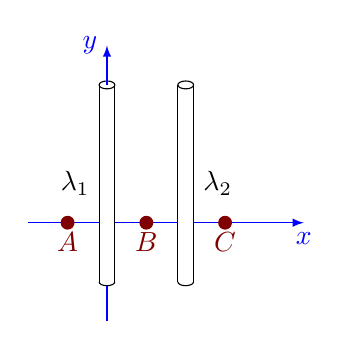
\begin{tikzpicture}[scale=0.5]
    \draw (0,3.5) ellipse (0.2 and 0.1);
    \draw (0,-1.5) +(180:0.2 and 0.1) arc (180:360:0.2 and 0.1);
    \draw [black] (-0.2,-1.5)--(-0.2,3.5) node[midway, left] {$\lambda_1$};
    \draw [black] (0.2,-1.5)--(0.2,3.5);
    \draw (2,3.5) ellipse (0.2 and 0.1);
    \draw (2,-1.5) +(180:0.2 and 0.1) arc (180:360:0.2 and 0.1);
    \draw [black] (1.8,-1.5)--(1.8,3.5);
    \draw [black] (2.2,-1.5)--(2.2,3.5) node[midway, right] {$\lambda_2$};
    \draw [blue, -{latex}] (2.2,0)--(5,0) node[below] {$x$};
    \draw [blue] (0.2,0)--(1.8,0);
    \draw [blue] (-2,0)--(-0.2,0);
    \draw [blue, -{latex}] (0,3.5)--(0,4.5) node[left] {$y$};
    \draw [blue] (0,-2.5)--(0,-1.6);
    \fill [red!50!black](-1,0) circle(5pt) node[below] {$A$};
    \fill [red!50!black](1,0) circle(5pt) node[below] {$B$};
    \fill [red!50!black](3,0) circle(5pt) node[below] {$C$};
  \end{tikzpicture}
  \captionof{figure}{Problema \ref{p:potencial05}\label{f:potencial05}}
\end{center}
\end{minipage}
%
\begin{Exercise}
  Se tiene un cilindro conductor muy largo de radio $a = \SI{1}{\centi\metre}$, con densidad superficial de carga uniforme $\sigma = \SI{1}{\micro\coulomb/\metre\squared}$, rodeado por un cilindro conductor hueco de radio interior $b = \SI{2}{\centi\metre}$ y radio exterior $c = \SI{2.5}{\centi\metre}$, con carga neta cero. \textit{a}) Determine la densidad superficial de carga en las superficies del cilindro exterior. \textit{b}) Calcule la diferencia de potencial entre la superficie exterior del cilindro hueco y un punto afuera del cilindro, a una distancia de $\SI{4}{\centi\metre}$ de su superficie. \textit{c}) Repita los cálculos pero ahora considerando que el cilindro hueco tiene una densidad de carga neta $\lambda = \SI{0.3}{\micro\coulomb/\metre}$.
\end{Exercise}
\begin{Answer}
  \begin{minipage}[t]{.4\textwidth}
    \textit{a}) $\SI{-0.5}{\micro\coulomb/\metre\squared}$ en la superficie interior y $\SI{0.4}{\micro\coulomb/\metre\squared}$ en la superficie exterior\\ \textit{b}) $|\Delta V| = \SI{1080}{\volt}$\\ \textit{c}) $\SI{-0.5}{\micro\coulomb/\metre\squared}$ en la superficie interior, $\SI{12.4}{\micro\coulomb/\metre\squared}$ en la superficie exterior y $|\Delta V| = \SI{33540}{\volt}$
  \end{minipage}
\end{Answer}
%
\begin{Exercise}
  Considere una espira circular de radio $R$, cargada con densidad lineal de carga uniforme $\lambda$. \textit{a}) Verifique que el potencial eléctrico en un punto $P$ situado a una altura $z$ del eje de la espira es:
  \begin{flalign*}
    V_P &= \dfrac{R\lambda}{2\varepsilon_o\sqrt{R^2+z^2}}
  \end{flalign*}
  \textit{b}) Verifique el resultado del campo eléctrico en ese punto obteniendo el gradiente del potencial.
\end{Exercise}
%
\begin{Exercise}
  Verifique que el potencial en un punto $P$ sobre el eje de un disco plano, a una distancia $z$ del centro del mismo, si el radio del disco es $R$ y la densidad superficial de carga es $\sigma$ es:
  \begin{flalign*}
    V_P &= \dfrac{\sigma}{2\varepsilon_o} \left ( \sqrt{R^2+Z^2} - Z \right )
  \end{flalign*}
\end{Exercise}
%
\begin{Exercise}\label{p:potencial06}
  Para la barra mostrada en la figura \ref{f:potencial06}, con densidad lineal de carga $\lambda$: \textit{a}) Verifique que el potencial eléctrico en el punto $P$ es:
  \begin{flalign*}
    V_P &= \frac{\lambda}{4 \pi \varepsilon_o} \ln \left ( \frac{a-L/2}{a+L/2} \right )
  \end{flalign*}
  b) Compruebe que en el caso $a \gg L$ se puede aproximar por:
  \begin{flalign*}
    V_P &\approx \frac{\lambda}{4 \pi \varepsilon_o} \frac{L}{a}
  \end{flalign*}
\end{Exercise}
%
\begin{center}
  \begin{tikzpicture}[scale=0.5]
    \draw (0,0) ellipse (0.1 and 0.2);
    \draw (-5,0) +(90:0.1 and 0.2) arc (90:270:0.1 and 0.2);
    \draw [black] (-5,0.2)--(0,0.2);
    \draw [black] (-5,-0.2)--(0,-0.2);
    \draw [blue, dotted] (0,0)--(5,0);
    \draw [blue, dotted] (-7,0)--(-5.1,0);
    % \draw [blue, dotted] (-2.5,0.2)--(-2.5,4);
    \draw [blue, dotted] (-2.5,-0.2)--(-2.5,-2);
    % \draw [black, -{Stealth}] (-12,0)--(-8,0) node[below] {$x$};
    % \draw [black, -{Stealth}] (-11,-1)--(-11,3.5) node[left] {$y$};
    \draw [blue, {Stealth}-{Stealth}] (-5,1)--(0,1) node[midway, above] {$L$};
    \draw [blue, {Stealth}-{Stealth}] (-2.5,-1)--(3,-1) node[midway, below] {$a$};
    \fill [blue](3,0) circle(5pt) node[above right] {$P$};
    % \fill [blue](-2.5,3) circle(5pt) node[above right] {$S$};
  \end{tikzpicture}
  \captionof{figure}{Problema \ref{p:potencial06}\label{f:potencial06}}
\end{center}
